\documentclass[../../main]{subfiles}

\renewcommand\thesection{\arabic{section}}


\begin{document}

\section{Plant Disease Detection} \label{sec:}

\begin{minipage} {0.62\textwidth}
    \vspace{-0.8cm}

    Developed and field-tested a TinyML-based plant disease detection system for
    rural West African farmers, enabling offline, low-cost inference. While
    slightly less accurate than cloud solutions, it outperformed them in
    accessibility and usability within local constraints.

\end{minipage}
\hfill
\begin{minipage} {0.35\textwidth}
    \begin{center}
        \vspace{-1.2cm}
        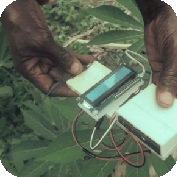
\includegraphics[width = 0.89\textwidth] {pics/disease_detection.pdf}
        \captionof{figure}[A farmer in Berekuso using the TinyML system.]{}
        \label{fig:case1Pic}
    \end{center}
\end{minipage}

\subsection{What They Did}

In this study\cite{ieee01africa}, researchers from Ghana develop a TinyML base plant
disease detection system based on ESP32 CAM. This was aimed to help the farmers
in Ghana to detect \emph{Brown Streak} and \emph{Mosaic} diseases in the
Cassava\footnote{Which is a common crop in West Africa.} plant. They held a comparative
study against the already available cloud based solution. Figure \ref{fig:case1Pic}
shows a farmer in Berekuso using the TinyML system.

\subsection{Results They Got}

The TinyML based system gave a \emph{promising performance} even though the
cloud based Plantix\footnote{Name of the app.} was better in terms of \emph{accuracy}.
But on an \emph{economic bases}, TinyML based system was \emph{more feasible} than the
cloud based one because inorder for the farmers to use the Plantix app they need to
afford a smartphone. Comparing to that the ESP32 based one was much cheaper.


\end{document}
